\chapter{Programming Languages and Linux commands}

Today's lecture will focus on programming languages and how to give a computer instructions through a command line. Programming languages allow programmers to write instructions, or \emph{code}, that can be interpreted by a computer to perform operations. However, computers cannot directly understand code. Instead, the code is translated to a format that the computer can understand. This process is called \emph{compilation}. When code is compiled, a program called a compiler takes the code as input, and as output produces operations that the computer hardware can directly execute.

%In Java that transformation is referred to as compilation. When Java code is compiled, a program called a compiler takes the Java code as input and as output produces code that’s easier for a computer to execute directly. \\

For instance, suppose that you have a text file with a large number of itemized expenses and you want to calculate the total cost of the expenses. To do this calculation, you could use a programming language to write code that instructs the computer to add up all of the expenses. This is more efficient than directly writing operations that the computer’s hardware can execute. \\ 

\section{Most popular programming languages}

Different programming languages are better for different applications. For example, some languages are better for making websites, while other languages are better for making mobile applications. \\

Java is one of the most popular programming languages. Java is used extensively by large companies like Oracle and Amazon. Java is also one of the primarily languages used to develop applications for the Android mobile operating system. \\

JavaScript is another very popular language. Despite its similarity to Java in name, JavaScript is a very different language from Java. JavaScript is one of the primary languages used for writing code to interact with browsers in websites, like Facebook or Google. 
%Javascript powers features of websites like generating dynamic content, sending requests to a server, making sure that the information entered in forms is correct, and many more things. 
%It’s also increasingly used to write applications. 
Javascript is a popular choice among newer and smaller companies. \\

Other programming languages that you might hear the names of include:
\begin{itemize}
\item \emph{Python}, \emph{Matlab}, and \emph{R}, three languages often used for scientific computing (e.g. mathematical modeling),
\item \emph{HTML} and \emph{CSS}, two languages used for writing websites; C++, one of the oldest/most common languages,
\item \emph{Assembly}, \emph{COBOL}, and \emph{Fortran}, three older languages that are behind a lot of old software (e.g. government software).
\end{itemize} 

The number and diversity of programming languages can be intimidating, but learning new programming languages languages becomes easier once you have a solid understanding of fundamental concepts. 
We recommend focusing on one programming language initially to learn fundamental concepts rather than spending time trying to learn multiple languages. \\

In this course we use one programming language, Java, to teach these fundamental concepts.
However, the ideas and concepts you learn will help you learn any programming language you need to. 
We use Java because it’s easier to learn, widely used, and illustrates many important concepts in programming. 40\% of developers who responded to a large survey of developers stated that they know Java! \\

\section{Overview of GUI and Command Line}

The two primary ways to interact with your computer are to either use a (1) Graphical User Interface (GUI), or (2) command line.

A \textbf{Graphical User Interface (GUI)} is the primary way most users of a computer interact with the computer. For example, the file explorer (Figure \ref{fig:windows:file}) is a GUI that provides an easy way for users to complete tasks on their computer. It is popular because users can use their mouse and intuitive commands to complete basic tasks. \\

\begin{figure}
	\centering
	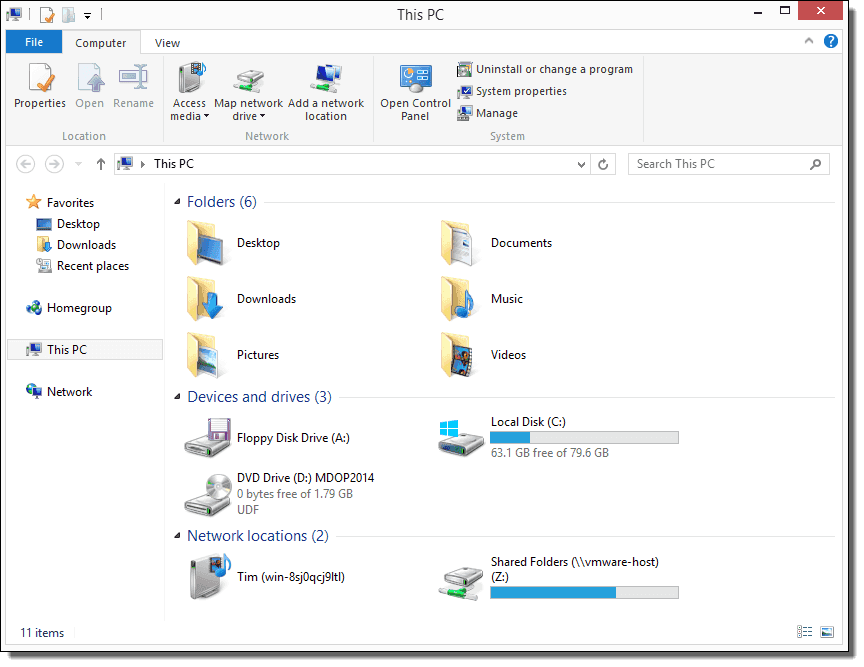
\includegraphics[width=0.85\textwidth]{images/windowsGUI.png}
	\caption{Windows file explorer}
	\label{fig:windows:file}
\end{figure}

The file explorer GUI hides the details of the operations being done by the computer away from the user of the program. This provides simplicity, but it also limits the flexibility of what a user can do with the computer. Moreover, it means that users can only interact with a system that has a GUI installed. This doesn’t include computers without a standard operating system, servers, or computers that a user is connected to remotely. \\

%The \textbf{command line} is a program you can access through the GUI of a linux machine. 
On the other hand, the \textbf{command line} is a program that  interface directly with the operating system and issue commands that it can understand. The command line can be accessed directly through the monitor without a GUI. In fact, before the invention of the GUI, the command line was the only way to interact with computers!  On modern computers, the command line can be accessed through the GUI of a linux machine. \\
%The command line is also installed on servers without a GUI and can be accessed directly through monitors (this was the only way to interact with computers before the invention of the GUI).\\

The command line allows the user to issue a broader range of commands and interact with computers without a graphical interface. 
%The command line lets users interface directly with the operating system and issue commands that it can understand. 
This increases the range of the commands that the user can issue, giving them more flexibility to perform complex and custom tasks. \\

\section{Linux command line}

We will discuss the command line used in the Linux operating system because it is one of the most common and intuitive command lines. \\

\begin{center}
    \begin{tabular}{| l | p{75mm} | }
      \hline
      Command & Description \\ \hline
      ls & List all the files in the current directory \\ \hline
      touch & Create a new file \\ \hline
      cd [name] & Changes the current directory to [name] \\ \hline
      mkdir [name] & Create a new directory within the current directory named [name] \\ \hline
      man [command] & Display the manual for a [command] \\ \hline
      cat [file] & Display the contents of [file] in the terminal \\ \hline
      mv [file] [location] & Moves [file] to the directory [location]. \\ \hline 
%      By default it moves file to a different name within the same directory. \\ \hline
      cp [file] [location] & Creates a new file with identical contents to the [file] specified in a new [location]. If a path for the file isn’t given, it will make a copy of the file in the same directory. \\ \hline
    \end{tabular}
\end{center}
  
  A folder in Linux is referred to as a \textbf{directory}. When you open a command line, you are located in a certain directory within the file system. All commands that you issue that relate to interacting with the file system like creating files, editing files, or renaming files will be issued in the context of this directory. This is like navigating to a particular folder within the GUI file explorer and completing all your operations relative to that folder.

\begin{figure}
	\centering
	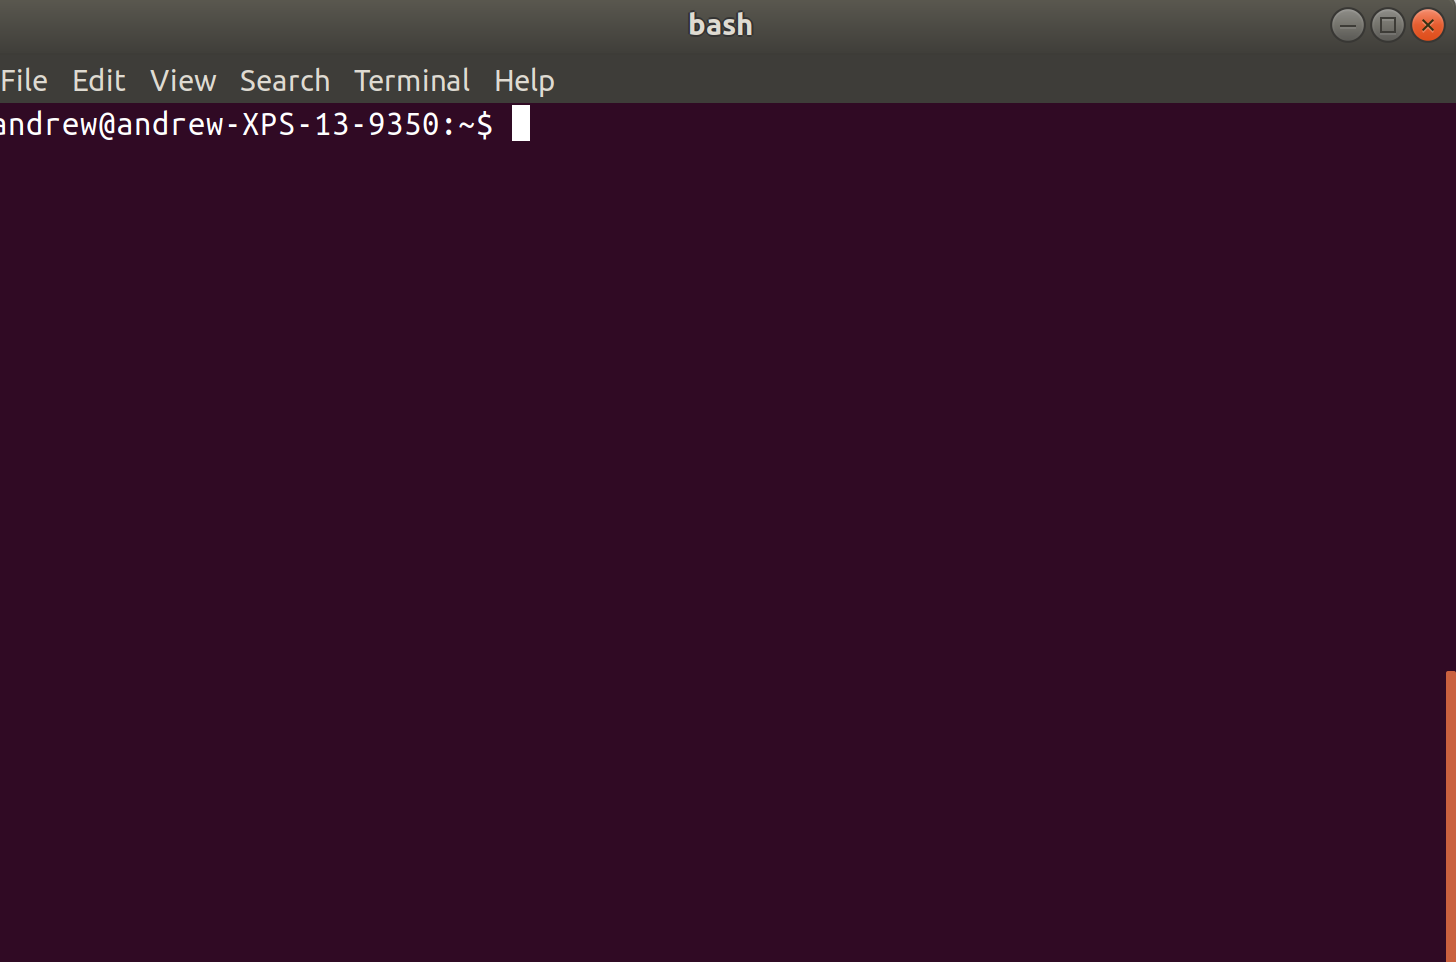
\includegraphics[width=0.85\textwidth]{images/commandLineOne.png}
	\caption{Linux command line}
	\label{fig:linux:one}
\end{figure}

Figure \ref{fig:linux:one} shows the command line interface for a Linux computer. The prompt shown is where the user can type commands. By default it prepends the user’s name, the name of the computer, and a dollar sign. The white rectangle represents the location of my cursor prompting the user to enter commands. \\

For example, Figure \ref{fig:linux:two} displays an example of creating a new directory called commandLineLearning (using the `mkdir` command) and then going inside the commandLineLearning directory (using the `cd` command). This is like making a new folder within an existing folder in the window’s file explorer, and then going inside that folder. \\

In Figure \ref{fig:linux:two}, the $\sim$ sign prepending the command represents the user’s home directory. The home directory is the outer most folder for that user’s account on the server or machine. \\

\begin{figure}
	\centering
	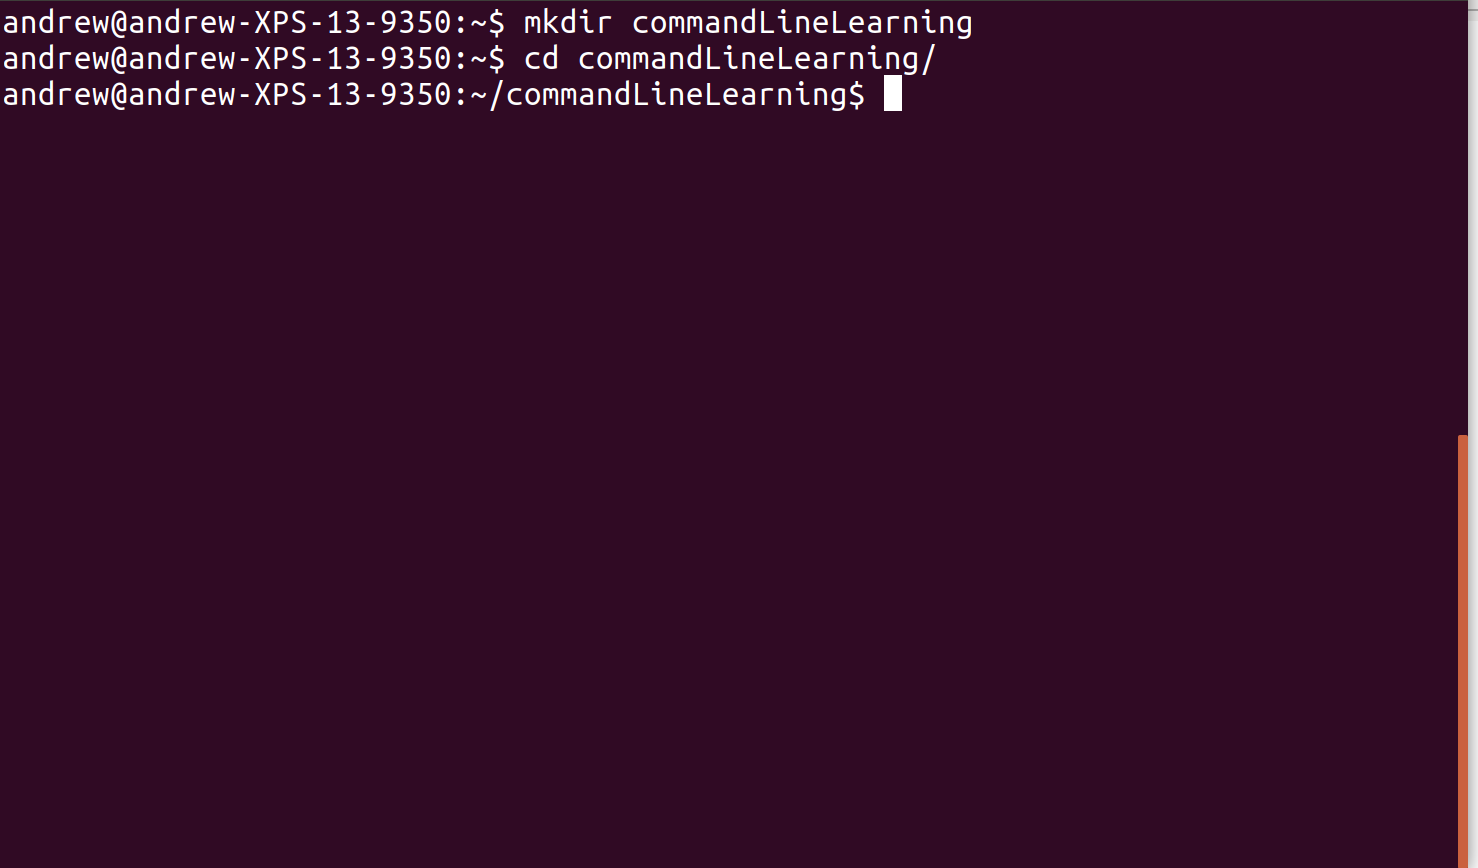
\includegraphics[width=0.85\textwidth]{images/commandLineTwo.png}
	\caption{Creating a directory}
	\label{fig:linux:two}
\end{figure}

\begin{figure}
	\centering
	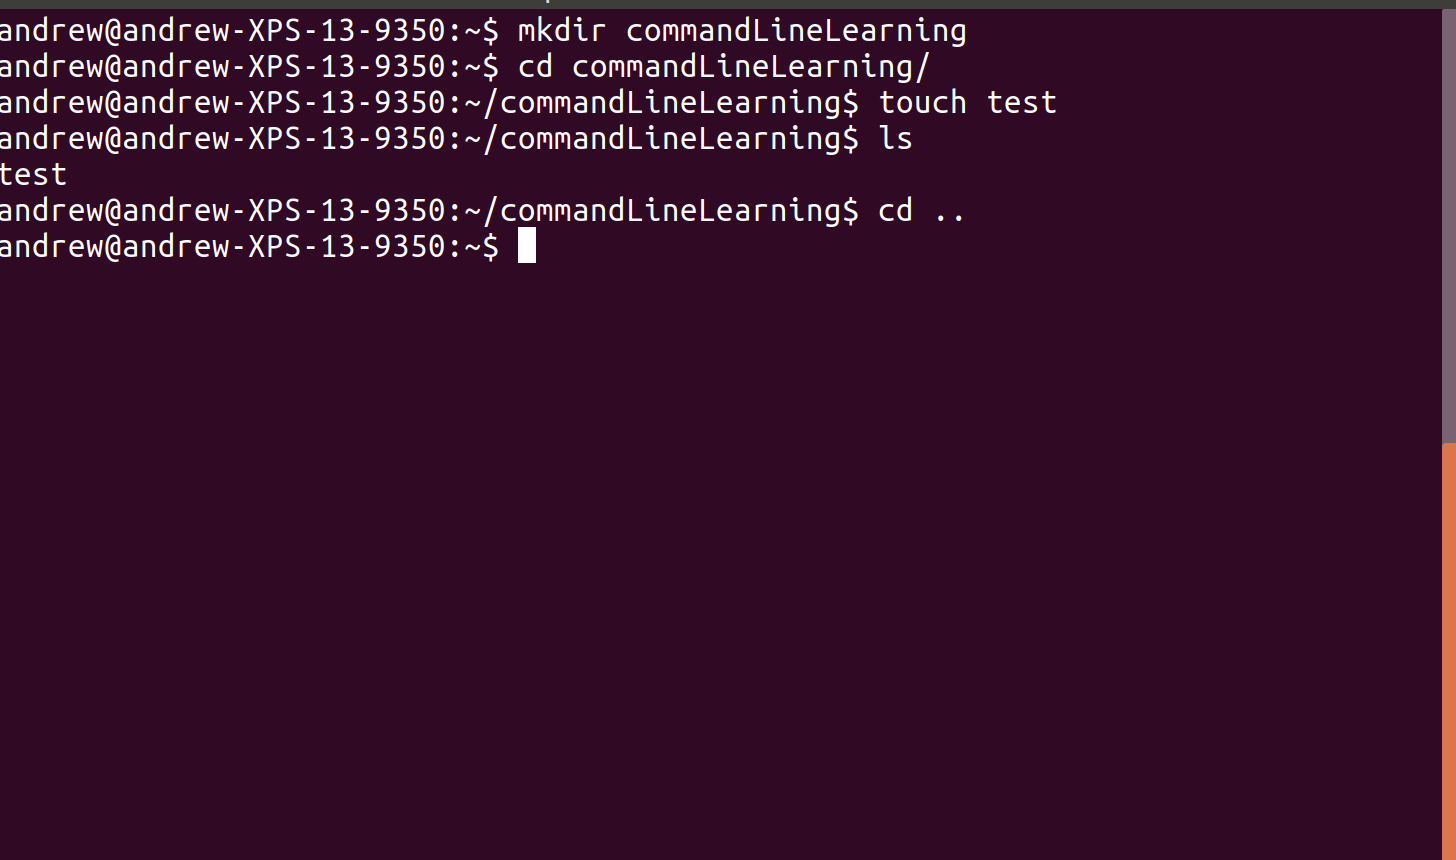
\includegraphics[width=0.85\textwidth]{images/commandLineThree.png}
	\caption{Listing files and navigating}
	\label{fig:linux:three}
\end{figure}

\begin{figure}[ht]
	\centering
	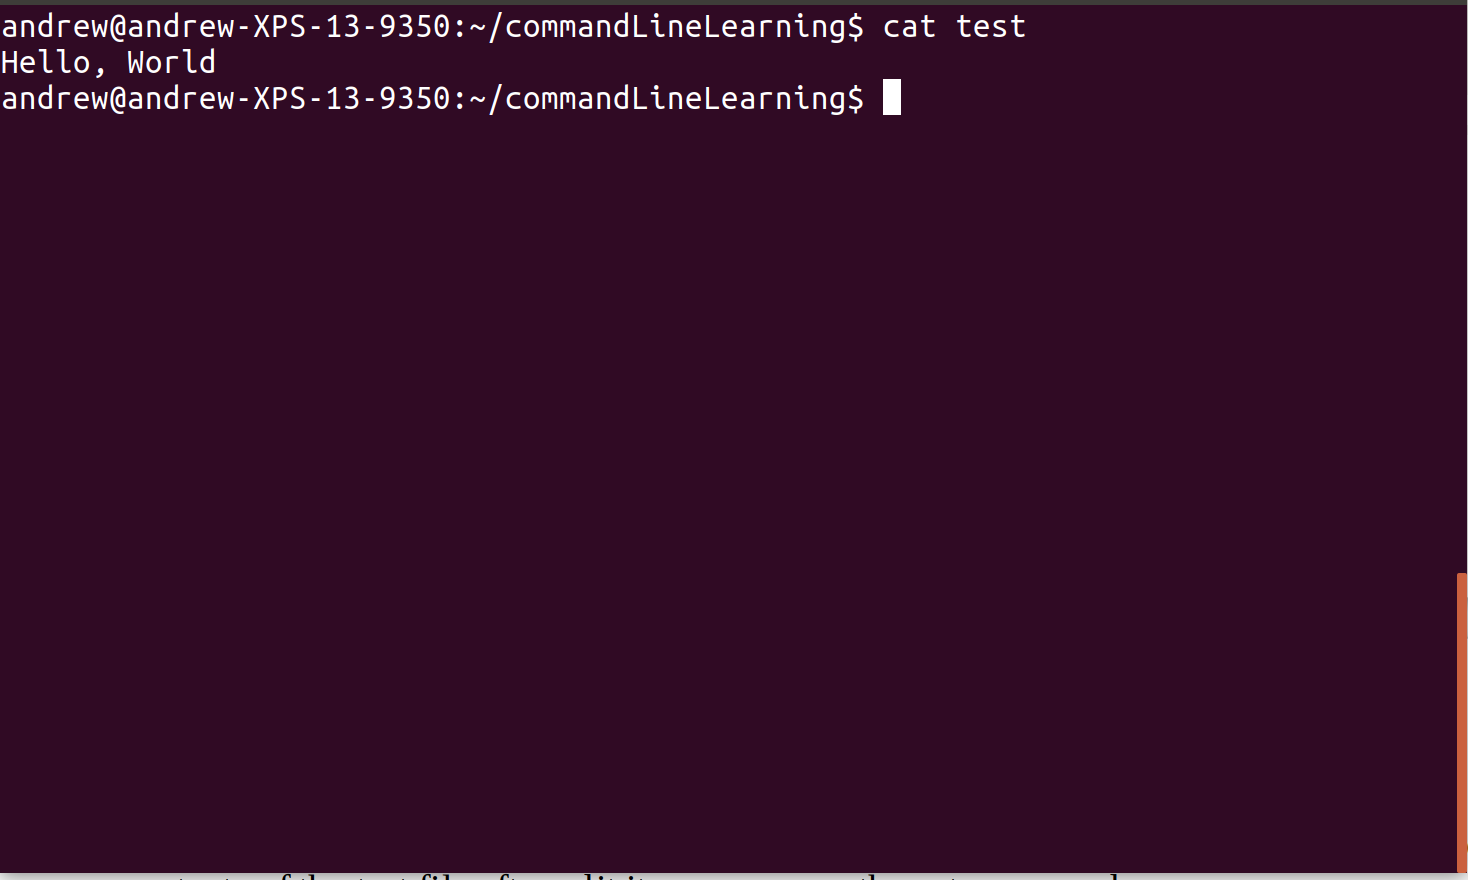
\includegraphics[width=0.85\textwidth]{images/commandLineFour.png}
	\caption{Cat command example}
	\label{fig:linux:four}
\end{figure}

If we want to create a file inside the commandLineLearning directory, we can use the ‘touch’ command to create a new file. If we want to see the files in the directory, we can use the ‘ls’ command to list all of the files inside the current directory. Finally, if we want to move back to the directory we were in before, we can use the ‘cd’ command with the parameters ‘..’ to move to the directory my current directory is contained within. In Linux, ‘..’ refers to the directory that contains the current directory, or the parent directory. These commands are summarized in Figure \ref{fig:linux:three}. \\

Try these commands out! You can edit the contents of test using any file editing software. To view the contents of the test file after you edit it, you can use the `cat` command (Figure \ref{fig:linux:four}). \\

%\newpage

\section{Lab: Running Hello World in the Command Line}

In this exercise, we will create a ``Hello World'' program in Java and run it --- only using the command line.

\begin{enumerate}
\item 
First, open the command line. 
\item Run the command \codeblock{cd $\sim$} which will move you to inside the \codeblock{$\sim$} folder. The \codeblock{$\sim$}  folder refers to your home directory.
\item
Next run \codeblock{cd Desktop}. This will take you to your Desktop. Afterwards, run \codeblock{cd CS103}, which will take you to your CS103 folder from Chapter 2. See Figure \ref{fig:linux:exercise:zero2}.

After running these commands, you might notice that the left side of your window (before the \$ sign) changes. This is because it indicates your current directory, which has changed from \codeblock{Desktop} to \codeblock{CS103}.

\begin{figure}[ht]
	\centering
	
\includegraphics[width=0.85\textwidth]{images/commandLineExercise_zero2}
	\caption{Navigating to the \codeblock{CS103} folder you created from Chapter 2.}
	\label{fig:linux:exercise:zero2}
\end{figure}

\item
Next, run \codeblock{mkdir Chapter\_8}. This will create a folder called \codeblock{Chapter\_8} inside the \codeblock{CS103} folder. 

To check that you created this folder, run \codeblock{ls}. This will show all of the contents in your current folder. Verify that \codeblock{Chapter\_8} is listed. See Figure \ref{fig:linux:exercise:one2}.

\begin{figure}[ht]
	\centering
	
\includegraphics[width=0.85\textwidth]{images/commandLineExercise_one2}
	\caption{Creating and going inside the \codeblock{Chapter\_8} folder.}
	\label{fig:linux:exercise:one2}
\end{figure}

\item 
Then run \codeblock{cd Chapter\_8}. This will take you inside the \codeblock{Chapter\_8} folder.

\item
Next, we will copy the Hello World file we created in Chapter 2 into the \codeblock{Chapter\_8} folder we just created.

To do this, run the command 

\codeblock{cp ~/Desktop/CS103/Chapter\_2/HelloWorld.java ~/Desktop/CS103/Chapter\_8/}

To understand why this command works, recall that running \codeblock{cp [file] [location]} makes a copy of \codeblock{[file]} in \codeblock{[location]}. In the cp command above, \codeblock{[file]} is the path to the Hello World file from Chapter 2, and \codeblock{[location]} is the \codeblock{Chapter\_8} folder you just created.

To check that the \codeblock{cp} command worked successfully, run the \codeblock{ls} command. This will display all of the files in your current folder, which is the \codeblock{Chapter\_8} folder. You should see a file called \codeblock{HelloWorld.java}. See Figure \ref{fig:linux:exercise:two2}.

\begin{figure}[ht]
	\centering
	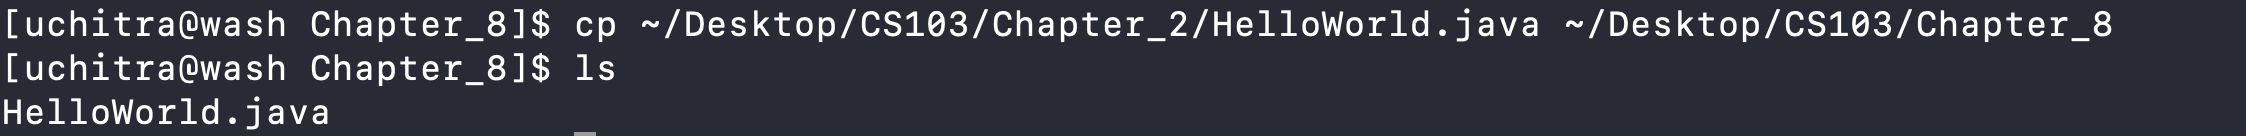
\includegraphics[width=0.85\textwidth]{images/commandLineExercise_two2}
	\caption{Copying the HelloWorld.java file from Chapter 2 into your \codeblock{Chapter\_8} folder.}
	\label{fig:linux:exercise:two2}
\end{figure}

\item
To verify that your code matches what you wrote in Chapter 2, run \codeblock{cat HelloWorld.java}. This will print out the contents of \codeblock{HelloWorld.java}.  See Figure \ref{fig:linux:exercise:three2}.

\begin{figure}[ht]
	\centering
	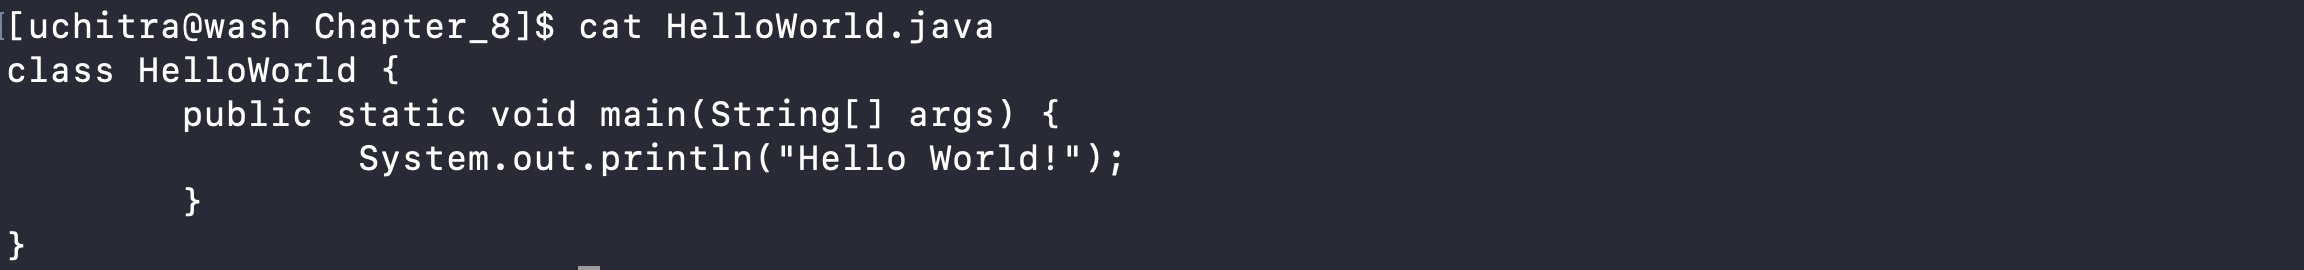
\includegraphics[width=0.85\textwidth]{images/commandLineExercise_three2}
	\caption{Running \codeblock{cat HelloWorld.java} to see the contents of \codeblock{HelloWorld.java}. Your code may look different depending on what you did in Chapter 2.}
	\label{fig:linux:exercise:three2}
\end{figure}

\item Now let's run our Hello World code! First, we have to compile the java file by running \codeblock{javac HelloWorld.java}. This will create a file named \codeblock{HelloWorld.class}. This file contains the bytecode instructions for the computer to run our program. See Figure \ref{fig:linux:exercise:four2}.

\begin{figure}[ht]
	\centering
	
\includegraphics[width=0.85\textwidth]{images/commandLineExercise_four2}
	\caption{Running \codeblock{javac HelloWorld.java}. Running \codeblock{ls} afterwards shows that a \codeblock{HelloWorld.class} file was created.}
	\label{fig:linux:exercise:four2}
\end{figure}

\item Next, run \codeblock{java HelloWorld}. Here, the \codeblock{HelloWorld} refers to the name of the ``class" in the java file. If everything is correct, the result should be the phrase ``Hello World!", as shown in Figure \ref{fig:linux:exercise:five2}.

\begin{figure}[ht]
	\centering
	
\includegraphics[width=0.85\textwidth]{images/commandLineExercise_five2}
	\caption{Running \codeblock{java HelloWorld.java}. The output of our program, which prints ``Hello World!", should appear below.}
	\label{fig:linux:exercise:five2}
\end{figure}

\item Congrats! You finished the lab! If you have extra time, check if someone sitting nearby needs any help.

\end{enumerate}
\newpage
\exercisesection

\begin{exercise}
Name three different programming languages.
\end{exercise}

\begin{exercise}
Name the process that turns your code into instructions that a computer can execute.
\end{exercise}

\begin{exercise}
Name an example of a GUI.
\end{exercise}

\begin{exercise}
Which command in the command line lets you to create a new directory?
\end{exercise}

\begin{exercise}
Which command in the command line lets you view the contents of a file?
\end{exercise}

\referencessection

Stack Overflow Developer Survey 2019. (n.d.).